




\chapter{Basics} \label{chap: basics}
This chapter lays the foundations to understand this thesis. First, \acrfull{md} as simulation method is introduced. Following, the basics of \acrshort{fem} and the used tools are presented. The last section outlines the theoretical process behind the optimisation algorithm used in this thesis.

\section{Molecular dynamics} \label{sec: MDBasics}
Adhesive bonding is an increasingly popular joining technique due to its applicability for composite materials, and their beneficial loading properties \cite{campilho_extended_2011}, \cite{pramanik_joining_2017}. Broader applicatio requires depends on a profound understanding of their material behaviour. For investigations at the atomistic level \acrfull{md} is a widely used approach  \cite{ries_mechanical_2024}. From the interactions with neighbouring atoms, Newton's equation is solved for every atom. These interactions are modelled via potentials. Non-bonded interactions such as van der Waals potentials are considered within a cutoff radius. The total potential energy of the system helps to identify the acting forces and accelerations of each particle. To follow the movements of the particles, time integration is necessary. Typical time step sizes are in the femtoseconds range, which makes only small time scales possible with reasonable computational costs \cite{ries_mechanical_2024}. Similar restriction holds for the system size, due to the increasing number of interactions with increasing domain dimensions. However, small dimensions lead to large surface-to-volume ratios which result in significant free surface effects. To avoid them, \acrfull{pbc} are used. They constrain the simulated volume as if it were integrated in an infinitely large domain. Regarding  particle tracking, a particle that leaves the system at one surface enters the system at the opposite surface. For the deformation of the whole volume element, the \acrshort{pbc} restrict in such a way that parallel surfaces remain parallel during the loading procedure. These boundary conditions result in a simulation of an infinitely long concatenation of the same volume element in each direction \cite{gorbunov_periodic_2022}.
With these adaptations the results from \acrshort{md} simulations can be transferred to a larger system. 
Thus, \acrshort{md} simulations allow building samples with prescribed properties followed by deformation tests to study the material behaviour \cite{buyukozturk_structural_2011}. 

\paragraph{Constitutive models}
During a deformation test stress and strain values are measured for every simulation time step. This leads to discrete points describing the stress and strain evolution over the loading process. To deduce general stress-strain curves from these discrete points, a mathematical expression is required. This is achieved through constitutive models, which describe the general qualitative relationship between stresses and strains \cite{mergheim_lecture_nodate}. Material specific properties are considered through material parameters.
Depending on the deformation regime for which the constitutive model holds, different material parameters are useful. Polymers are usually modelled with elastoplastic models. Elastoplastic models combine two characteristic material behaviours – elasticity and plastification. An elastic process is characterised by the fact that the loading process is reversible. This means, the loading and unloading processes follow the same path in a stress-strain diagram \cite{mergheim_lecture_nodate}. Generally, the path can follow any function. In combination with plastification, usually linear elastic behaviour is assumed (QUELLE), which can be specified with the material parameters Young's modulus $E$ and Poisson's ratio $\nu$. An elastoplastic material behaves linear-elastic until a stress limit is reached. After that so-called yield stress $\sigma_0$, the material response is irreversible, which leads to the exemplary stress-strain function in \autoref{fig:elastoplasticityCurve} \cite{mergheim_lecture_nodate}. The loading path in the plastic regime can be described by various functions. In the scope of this work, we focus on hardening functions, where the stress increases with increasing plastic strain (QUELLE). They describe the material behaviour in the plastic regime through multiple plastic material parameters. An important property of elastoplastic material models is their rate-independence. This characteristic leads to identical material behaviour under loading processes with varying strain rates. However, this assumption is not valid for materials with viscous properties. The material response of polymers can include viscous parts as well, meaning their behaviour can be rate-dependent. If an elastoplastic constitutive model is to be used, an adequate procedure must be employed to filter out the viscous component of the material response. 


\begin{figure}[H]
    \centering
    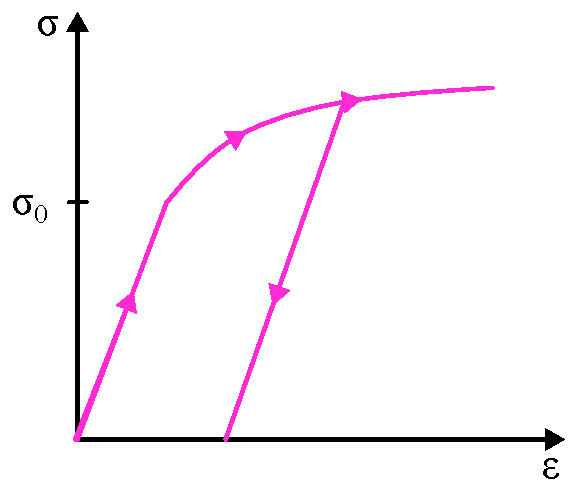
\includegraphics[width=0.5\textwidth]{elastoplasticityCurve.pdf}
    \caption{Exemplary stress-strain curve for elastoplastic materials based on \cite{mergheim_lecture_nodate}}
    \label{fig:elastoplasticityCurve}
\end{figure}


% Elastoplastic models are used for materials, which show elastic characteristics until a yield strength is reached. 

% However, this is only possible, if the viscous parts are neglected. (NUR WEIL VISCO WEGGELASSEN WIRD) In the elastic regime the material  parameters  Young's modulus $E$ and Poisson's ratio $\nu$ are used to specify the material. They show elastic behaviour until a yield strength is reached. 
% Then, the plastification begins which can be described by various hardening models depending on the material characteristics \cite{mergheim_lecture_nodate}. 

\paragraph{Previous work}
This work focusses on the investigations by \citet{ries_deciphering_nodate}, who studied the curing and deformation properties of epoxy through \acrshort{md} simulation. They developed models with numerous mixing ratios of resin and hardener\footnote{The mixing ratio is specified in the notation resin:hardener}. Their deformation tests build the motivation for the optimisation process here developed. \citet{ries_deciphering_nodate} conducted uniaxial tensile tests loading a sample with linear strain up to a maximum value of 20 \%. The test sample is constrained by \acrshort{pbc}, which allow lateral contractions. To record the stress-strain response without viscous effects they developed a procedure to approximate the quasi-static material response. Then only elastic and plastic reactions are considered. Their choice of constitutive models is based on the assumption of isotropic material behaviour. To describe the elastic material behaviour they used the Neo-Hookean hyperelasticity model. The plastic reactions are modelled via the VOCE-model which defines the stresses during the hardening process through \cite{voce_practical_1948}.

\begin{equation} \label{eq: voce}
    \sigma = \sigma_0 + \alpha(1 - \text{exp}(-\beta \varepsilon_{pl})) + \gamma \varepsilon_{pl}
\end{equation}
\begin{gather*}
    \sigma_0: \text{ Yield stress} \\
    \varepsilon_{pl}: \text{ Plastic strain} \\
    \alpha, \beta,  \gamma: \text{ Hardening parameters}
\end{gather*}


Together with the elastic material parameters Young's modulus $E$ and Poisson's ratio $\nu$, six constitutive parameters are available to fit the stress-strain pairs measured through \acrshort{md} simulation. Their values are calculated using an external minimisation algorithm. The detailed procedure is described in \cite{ries_deciphering_nodate}. The procedure of \citet{ries_deciphering_nodate} is important since their data are used for the model assessment of the optimisation procedure developed in this work. A detailed description of the optimisation setup is given in \autoref{chap: modelsAndMethods}. In the verification studies the optimisation procedure is tested with mixing ratios 4:3, 6:3 and 8:3. To evaluate its performance the \acrlong{omp} are compared to the material parameters obtained by \citet{ries_deciphering_nodate}. However, a valid comparison requires two conditoins: first, that stress-strain data are collected under similar loading conditions, – and – second, that the same constitutive model is used to determine the material parameter values. Therefore, a detailed understanding of the methods used by \citet{ries_deciphering_nodate} is essential, since they are adopted for the simulation process used in this work.  



\section{Finite Element Method} \label{sec: FEMBasics}

The \acrfull{fem} is a widely used approach for XXX. 
The purpose of \acrshort{fem} is to find solutions for field problems in complex regimes \cite{willner_vorlesungsskript_nodate}. However, an analytical solution is only possible for simple problem formulations. Therefore, in \acrshort{fem} the regime is discretized into a finite number of elements. The element behaviour is characterised by approximation functions with a finite number of parameters. Assembling the approximation functions of all elements, leads to an equation system that approximates the solution for the whole regime \cite{jagota_finite_nodate}. The \acrshort{fem} is primarily used in structural mechanics to provide information about forces and deformations. The general procedure of the \acrshort{fem}, based on \citet{willner_vorlesungsskript_nodate} and \citet{steinke_finite-elemente-methode_2015}, is presented in the following: 
\begin{align*}
    &\text{1. Discretisation} \\
    &\text{2. Construction of stiffness matrix}\\ 
    &\text{3. Coordinate transformation} \\
    &\text{4. Assembly} \\
    &\text{5. Application of boundary conditions} \\
    &\text{6. Solving equation system}
\end{align*}

In the first step, we discretise the continuum in finite elements. The shape and size of the elements depend on the geometry of the regime, and the required level of precision. To achieve more accurate solutions, smaller elements are necessary. Next, a local stiffness matrix $\boldsymbol{K}$ is created for every which connects the acting forces $\boldsymbol{S}$ with the element deformations $\boldsymbol{u}$ via 
\begin{equation}
    \boldsymbol{S} =  \boldsymbol{K} \cdot \boldsymbol{u}.
\end{equation}
Although the equation holds for an element, the calculated forces and deformations are defined at the element nodes. The entries in the stiffness matrix depend on the  element type used. They contain material-specific information defined by material parameters. The stiffness matrices were constructed in local coordinate systems. To connect them, a transformation into a global system is necessary. In the fourth step, the equation systems of all elements are combined into a global matrix system. In the assembly, neighbouring elements share their nodes, which needs to be considered during the construction of the equation system. Through prescribed loadings at the boundary of the continuum, certain forces or deformations are known. They are inserted in the equation system as boundary conditions. In the final step the equation system is solved yielding the deformations for every node \cite{willner_vorlesungsskript_nodate}, \cite{jagota_finite_nodate}. 

\paragraph{Application}
A main advantage of \acrshort{fem} is its high flexibility. Many different geometries can be modelled through appropriate choice of element shapes. The accuracy can be adjusted with the element size. Decreasing element sizes lead to more accurate results but require higher computational effort. However, \acrshort{fem} simulations are normally quite fast, since the computations are performed on easy element geometries. In addition, multiple commercial tools are available to construct a \acrshort{fem} simulation. They offer multiple options to define the properties throughout the entire procedure, which makes them applicable for a wide range of problems. \\
As described in XXX, the aim of this work is to create a new procedure to determine the material parameters of materials, investigated with \acrshort{md} simulations. Since a \acrshort{fem} simulation requires significantly less computational effort whilst still producing sufficiently accurate results, we decided to base this work on \acrshort{fem}. Therefore, the model used in the \acrshort{md} simulations must be transferred into a \acrshort{fem} model. As reference, we use the \acrshort{md} simulations performed by \citet{ries_deciphering_nodate}. To achieve this, we must transfer their model properties and testing conditions into a \acrshort{fem} simulation environment. In particular, the material behaviour, the boundary conditions, and the applied load must be transferred as exactly as possible. A description of the implementation is given in \autoref{chap:modelsAndMethods}.


%  To describe the material behaviour, we use the constitutive model \citet{ries_deciphering_nodate} selected for the material parameter search. 

%  - transfer material parameters in continuum
%  - transfer EasyPBC
%  - transfer load applications
%  - homogenous behaviour: fast simulation 
%  --> then much faster 

% accurate simulation of mat behav and gleichzeitig mat params 
% alle werte lassen sich direkt auslesen 
% lässt 

% there are cases, where this state is not fully correct. 
% - various geometries possible
% - fast simulation time
% - easy to use in programs
% - high felxibility --> various constitutitve models voreingestellt
% - choose const model --> define material parameters 
% - or define material behaviour through exp data (if mat par not known, exact const model not impemented)
% - mesh part: denepends on geometry --> el type and sizes
% - apply bc 
% - possible to read out all stress and strain values
% - differente element types
% - fieldOutput: different vaiables which describe reactions (Energy, Stress,s train, deformation, etc)
% - FO in all directions available
% - per loadstep
% - decided for FEM because:
% - fast
% - direct results for material response - material parameter relation
% - easy to construct (for case of cube)
% - load step erklären


\section{ABAQUS Scripting Interface} \label{sec: AbaqusBasics}

The task addressed in this thesis was implemented using \name{Abaqus}/\acrshort{cae} 2024. The commercial software is a widespread tool for \acrshort{fem} analysis. At the Institute of Applied Mechanics (LTM) of the FAU, the software is frequently used, which simplifies subsequent works with the program. In addition, \name{Abaqus} has an integrated \name{Python}-based scripting tool called "Abaqus Scripting Interface". It works as an \acrfull{api} to use the object-oriented programming language \name{Python} in the \name{Abaqus} environment \cite{dassault_systems_abaqus_2015-1}. The "Abaqus Scripting Interface" allows access to the functionalities of \name{Abaqus}/\acrshort{cae} from scripts. Functions, such as the creation and modification of models and jobs, can be controlled via code. Additionally, the output data written for successful executed jobs can be processed \cite{dassault_systems_abaqus_2015-1}. Since it is a \name{Python} extension, the standard programming functionalities are also available. The integration of \name{Abaqus} functionalities in a standard program structure, makes the "Abaqus Scripting Interface" the perfect tool for the task of this work. Due to this property, the realisation of the project is possible in a single script whose structure is shown in \autoref{chap: modelsAndMethods}. The implementation permits a parameter-based analysis which makes value adaptations very fast and easy. If these parameter values are stored in an input file, the user only needs to modify this file without changing the code in the script. This enables fast parameter studies with multiple values. This feature is used in this work to test multiple combinations of material parameters.  



% These possibilities enable a wide range of applications 

% - use abaqus because of XXX
% no reasion> bei eva abschreiben
% - python scripting -> user guide zitieren
% - python script führt befehle aus die klicks in Cui entpsrechen --> alle möglichkeiten die in gui auch vorhanden sind
% - alle funktionen von python vorhanden
% - objektorientierte programmierung möglich und parametrisierung --> deutlich schneller als mit gui
% - input file ist json file: einfach auszulesen, nur dies muss von user bearbeitet werden
% - 

\subsection{EasyPBC plugin} \label{subsec: EasPBC}

EasyPBC is an \name{Abaqus} plugin which automatically creates \acrshort{pbc}. The plugin is developed by \citet{omairey_development_2019}. It is not an official \name{Abaqus} extension, thus it is not available online. Due to its utilisation in previous works, the plugin was already in use at the institute. The \acrshort{pbc} must constrain parallel surfaces to remain parallel during deformation. To realise this property in \name{Abaqus}, EasyPBC generates node sets of the surface nodes. Opposing nodes are linked via constraint equations to couple their motion. In addition, reference points are created with each one linked to a surface. Therefore, applying load to a reference point causes corresponding reactions on the connected surface which is used for a simplified load application. 

% the entire surface can be loaded by applying a load at the corresponding reference point.  

% for every surface one corresponding reference point is created. The reference points are linked  


% REFERENCE POINTS FÜR LASTANGRIFF 

% - plane surfaces remain plane after deformation
% - wird auf knoten angewendet
% - displacement bc 
% - bei eva nachgucken
% - create PBCs auomatisch
% - needs elastic material parameters
% - reference points are connected to surfaces --> apply load homogeneous on surface



\section{Mathematical basics} \label{sec: mathematics}

To find the values of material parameters, that best fit the material behaviour measured in the MD-simulation, a mathematical formulation is necessary. This leads to an optimisation problem, where a calculated error, defined as an objective function of the material parameter values, should be minimised. We first discuss the numerical method to minimise the error, followed by the construction of the error value.

\subsection{Numerical optimisation} \label{subsec: numericaloptimisation}
To solve the optimisation problem various mathematical algorithms are available. We decided to use the Nelder-Mead algorithm, which is a widely used gradient-free optimisation algorithm \cite{gao_implementing_2012}. In a gradient-free algorithm, the derivatives of the function are neglected in the process. Our objective function is based on results of \acrshort{fem} analysis, which makes it impossible to determine its derivatives directly. Therefore, only gradient-free algorithms are applicable. In addition, ignoring the derivatives saves significant computational costs, which leads to fast convergence times \cite{pham_comparative_2011}. Due to its simple structure, the algorithm is a standard feature in many numerical libraries \cite{singer_efficient_2004}. In \name{python} it is available in the SciPy.minimize function. In \autoref{sec: optimisationCode} the function call is described in detail. Here we focus on the procedure of the algorithm, which is visualised in \autoref{fig:nelderMead}. The algorithm is capable of finding a local minimum of a scalar function depending on $n$ optimisation variables. In this work the optimisation variables are the material parameters. The definition of the objective function can be found in \autoref{chap: modelsAndMethods}. Assuming the objective function is known, the first step is to create $n+1$ points $\mathbf{P}$ in an $n$-dimensional space. In the initial step of the algorithm the positions of the points must be determined. This is done by an initial guess $\hat{x}$ for every optimisation variable. To process six optimisation variables, the initial guess would look like this: 
\begin{gather}
    \mathbf{\hat{x}} = [\hat{x}^0, \hat{x}^1, \hat{x}^2, \hat{x}^3, \hat{x}^4, \hat{x}^5] \\
    \text{with } \hat{x}^i \equiv \text{initial guess of the $i$-th optimisation variable}
\end{gather}

Based on this, the initial points $\mathbf{\hat{P}_i}$ are constructed. The first one is defined as $\mathbf{\hat{P}_1} = \mathbf{\hat{x}}$. For the other points, the value of one variable in the initial guess is changed each. The points are connected to each other in such a way that an $n$-dimensional simplex is created. A simplex is a general geometric object in $n$-dimensional space consisting of $n+1$ points.

The points result in an $n$ dimensional simplex. In the next step, the function values corresponding to the points $\mathbf{P_i}$ are evaluated and sorted by size. The highest function value $y_h$ maps the worst value combination $\mathbf{P_h}$ of the optimisation parameters. When the algorithm starts, a centroid of all points of the simplex except $\mathbf{P_h}$ is determined. At this point $\mathbf{P_C}$, $\mathbf{P_h}$ is reflected at a new position $\mathbf{P_R}$. Before the new point $\mathbf{P^{*}}$ is positioned, the corresponding function value $y(\mathbf{P_R})$ needs to be evaluated. Depending on its value, one of four possible operations is executed. As depicted in \autoref{fig:nelderMead}, \benennung{Reflection} is performed, if $y(\mathbf{P_R})$ is smaller than the second-worst function value. If $y(\mathbf{P_R})$ is even smaller than $y(\mathbf{P_0})$, which is currently the best value, \benennung{Expansion} is performed. In all other cases, a form of \benennung{Contraction} is executed. The worst case occurs, if both \benennung{Contraction} operations bring an increased function value $y(\mathbf{P^*})$ compared to $y(\mathbf{P_R})$ and $y(\mathbf{P_h})$. As a consequence, \benennung{Shrinking} the whole simplex towards the currently best position is the only possibility. To choose the correct operation depending on the current simplex, multiple evaluations of $y$ at different points $\mathbf{P}$ might be necessary. Thus, during one optimisation iteration, multiple function evaluations are accomplished. When an improved position $\mathbf{P^{*}}$ is found, the algorithm starts again with the new simplex \cite{nelder_simplex_1965}. \\

If the variations of the functions values $y_i$ fall below a certain limit, the minimum with its corresponding parameter values is found. To ensure a successful search the initial simplex should be scaled regularly \cite{baudin_nelder-mead_nodate} which is possible through a regular distribution of the points $\mathbf{\hat{P}_i}$ in space. This can be difficult if the values of the optimisation variables differ greatly in size. Therefore, it is necessary to normalize the variable values within the range of 0 to 1. The algorithm is vulnerable to becoming stuck in local minima due to the \benennung{Shrinking} operation \cite{luersen_globalized_2004}. Therefore, a smart choice of initial values is helpful, to avoid starting points near a local minimum. However, if the trend of the objective function is unknown, this can be challenging. In addition, the number of optimisation parameters should be constrained. So far, stable convergence behaviour of the Nelder-Mead algorithm has mostly been studied for small numbers of variables \cite{singer_efficient_2004}, \cite{pham_comparative_2011}.





% There are four possible operations to improve the position of $\mathbf{P_h}$. 

%  De

%  of $\mathbf{P_h}$ at the centroid are the first two. 

%  Only, if $y^{*}$ is smaller than $y_h$, $\mathbf{P^{*}}$ is set as new point $\mathbf{P_i}$ in the simplex. If $y^{*}$ is larger than $y_h$, the new point is even worse than $\mathbf{P_h}$. Therefore, the operations contraction or shrinking are performed. They should find a position $\mathbf{P^{**}}$ between $\mathbf{P_h}$ and its reflection $\mathbf{P^{*}}$, which leads to a better function value $y^{**}$. This needs multiple iterations because for every guess $\mathbf{P^{**}}$ the function needs to be evaluated. When a better function value is found, $\mathbf{P_h}$ is replaced by $\mathbf{P^{*}}$ or $\mathbf{P^{**}}$ and the algorithm starts again with the new simplex \cite{nelder_simplex_1965}. 
 
%  Therefore, multiple function evaluations are necessary during one iteration of the optimisation. 



\begin{figure}[H]
    \centering
    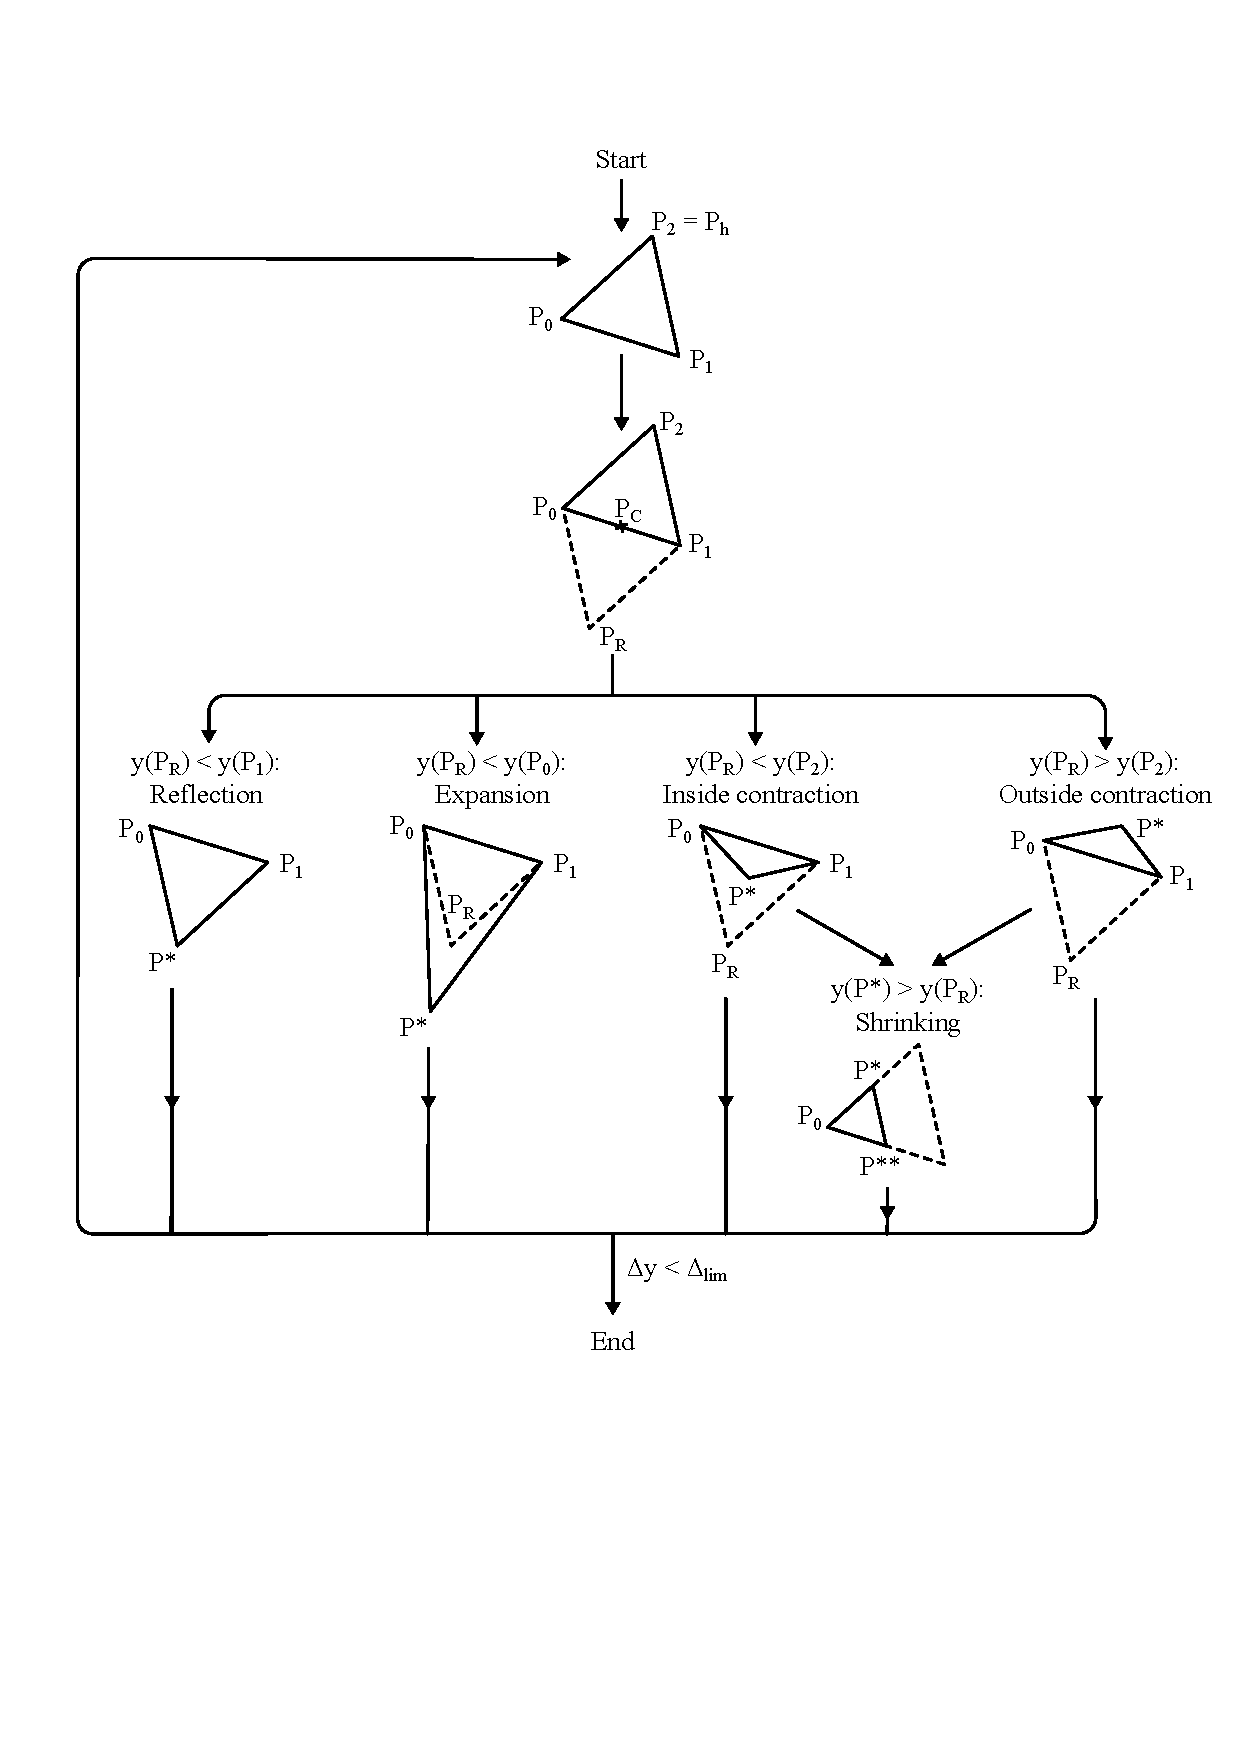
\includegraphics[width=0.8\textwidth]{NelderMeadAlg.pdf}
    \caption{Visulisation of the Nelder-Mead algorithm for three optimisation parameters }
    \label{fig:nelderMead}
\end{figure}

POSITION ZUM SCHLUSS ANPASSEN

\subsection{Root mean squared error} \label{subsec: RMSE}
To use the Nelder-Mead algorithm, we need to construct an objective function that returns a scalar value. It should be preempted at this point that several values must be minimised for an adequate optimisation result. In order to handle this issue, it is necessary to condense all applicable data into a single value. As a representative value we choose the \acrfull{rmse}. It is a frequently used value to express variations of two data sets - usually a reference data set $f$ and a test data set $\hat{f}$ \cite{morrow_method_2010}. The \acrshort{rmse} is based on the difference between the data points at position $i$. This deviation is composed for all points, and then combined in the following formula

\begin{equation} \label{eq: RMSE}
    \text{RMSE} = \sqrt{\frac{1}{N}\sum_{i=1}^{N} (f_i - \hat{f}_i)^2}
\end{equation}

With this definition, the proportion of all deviations in the \acrshort{rmse} is equal. The value of the \acrshort{rmse} is always positive and tends towards zero for perfectly matching data sets. In addition, the unit of the \acrshort{rmse} matches that of the data points (QUELLE). This characteristic is advantageous for the evaluation of its value. Since we must include the deviations between $M$ multiple data sets, we extend the formulation to 

\begin{equation} \label{eq: multiRMSE}
    \text{RMSE} = \sqrt{\frac{1}{M} \sum_{j=1}^{M} \left[ \frac{1}{N} \sum_{i=1}^{N} (f_i - \hat{f}_i)^2 \right] _j}
\end{equation}

The application of this formula in the developed code is explained in \autoref{sec: errorCalculation}.


%The numerical algorithm can only find adequate results, if the definition of the objective function is suitable. 

% verwendet weil:

% - fehler mitteln
% - alle werte mit einbeziehen
% - fehlereinheit in einheit der größe (wenn eine größe (stress oder strin) gemessen wird)
% - gilt nicht wenn stress und strain gemischt wird
% - most common
% - fehlr größe ist nicht quadriert 
% - - fitting über den gasmten kurvenverlauf --> alle punkte sollen gleich eingehen




% - have n varibales --> here 6 
% - create n+1 points in a n-dimensional space
% - function y 
% - P_i are the n1 points
% - y(P_i) are the function values from that we create a simplex
% - determine y_low and y_high (lowest and highset function values)
% - build centroid y_c between all points except y_high
% - then three options to replace y_high (which is the worst value)
% reflection: refelct y_high at y_c (Formel aus paper) is called y*
% - i y* is better than y_high we replace it 
% - if y* is better than y_low (we found a new minimum) we expand y* in the same direciton to y^{**}
% if y++ is better than y_low we replace y_h by y++
% - if not we reaplce y_h by y*
% contraction: if y* is is higher than all other y's (so we just found a value whcih is still the maximum), we chosse p_h or P* to be the new P_h 
% - then use contraction coefficient to find P** (inside or outside contraction)
% - if y** worse than y_high or y* --> shrink towards P_l 
% - stopping cruíterion: error smaller than defined value
% - simplex should not become too small compared to the curvature of the surface -> leads to small curvatures which lead to high variance in the estimates without finding accurate minimum
% - create intial simplex with x_0 as input --> macht SciPy irgendwie, angelbich nach irgendeiner logik 
% - intiial guess ist P_1(rray mit 6 variablen) dann wird durch den array iteriert und jeweils ein wert verändert und daraus der näcshte Oonkt P_i erzeugt -> jeweils nur veränderung einer variablen. 
% - scipy has dynmaic scaling how to variate the intial values





